\section{Implementation}
\label{sec:Implementation}

The design of iProbe is generic and platform agnostic, and works on native binary executables. 
We built a prototype on Linux which is a commonly used platform for service environments. 
In particular, we used a compiler technique based gcc/g++ compiler to implement the hook place holders on standard Linux 32 bit and 64 bit architectures. 
In this section we first show the implementation of the iProbe framework, and then discuss the implementation of FPerf a tool built using iProbe.

\subsection{iProbe Framework}
As we presented in the previous section, the instrumentation procedure consists of two stages.

\indent \textbf{ColdPatch}: In the first phase the place holders for hooks are created in the target binary. 
We implemented this by compiling binaries using the \texttt{-finstrument-functions} flag. 
Note that this can be done simply by appending this flag to the list of compiler flags (e.g., \texttt{CFLAG, CCFLAG, CXXFLAGS}) and most of cases it works without interfering with user code. 

In details this compiler option places function calls to instrumentation functions (\texttt{\_cyg\_profile\_func\_enter} and \texttt{\_cyg\_profile\_func\_exit})  after the entry and before the exit of every function. 
This includes inline functions (see second state in Figure \ref{fig:state_rep}). 
Subsequently, our ColdPatcher uses a binary parser to read through all the target binaries, and search and replace the instruction offsets containing the instrumentation calls with NOP instructions (instruction 90). 
Symbolic and debug information is read from the target binary using commonly available \texttt{objdmp} tools; 
This information combined with target instruction offsets are used to generate the probe list with the following information:
\begin{verbatim}
<Instr Offset, Entry\Exit Point, Meta-Data>
\end{verbatim}
The first field is the instruction offset from the base address, and the second classifies if the target is an entry or an exit point of the function. 
The meta-data here specifies the file, function name, line number etc. 

\indent \textbf{HotPatching}: 
In the run-time phase, we first use the library interposition technique, \texttt{LD\_PRELOAD}, to preload the instrumentation functions in the form of a shared library to the execution environment. 
The HotPatcher then uses a command line interface which interacts with the user and provides the user an option to input the target process and the probe list.
Next, iProbe collects the base addresses of each shared library and the binary connected to the target process from \texttt{/proc/pid/maps}.
The load address and offsets from the probe-list are then used to generate a hash of all possible probing points. 
iProbe then use the meta-data information to provide users a list of target functions and their respective file information.  
It takes as input the list of targets and interrupts the target process. 
We then use \texttt{ptrace} functionality to patch the target instructions with calls to our instrumentation functions, and release the process to execute as normal.
The instrumentation from each function is registered and logged by a shared memory logger. 
To avoid any locking overhead, we have a race free mechanism which
utilizes thread local storage to keep all logs, and a buffered logging mechanism.

\subsection{FPerf: An iProbe Application for Hardware Event Profiling}
\label{sec:imp:configure}


\begin{figure}[t]
    \begin{center}
      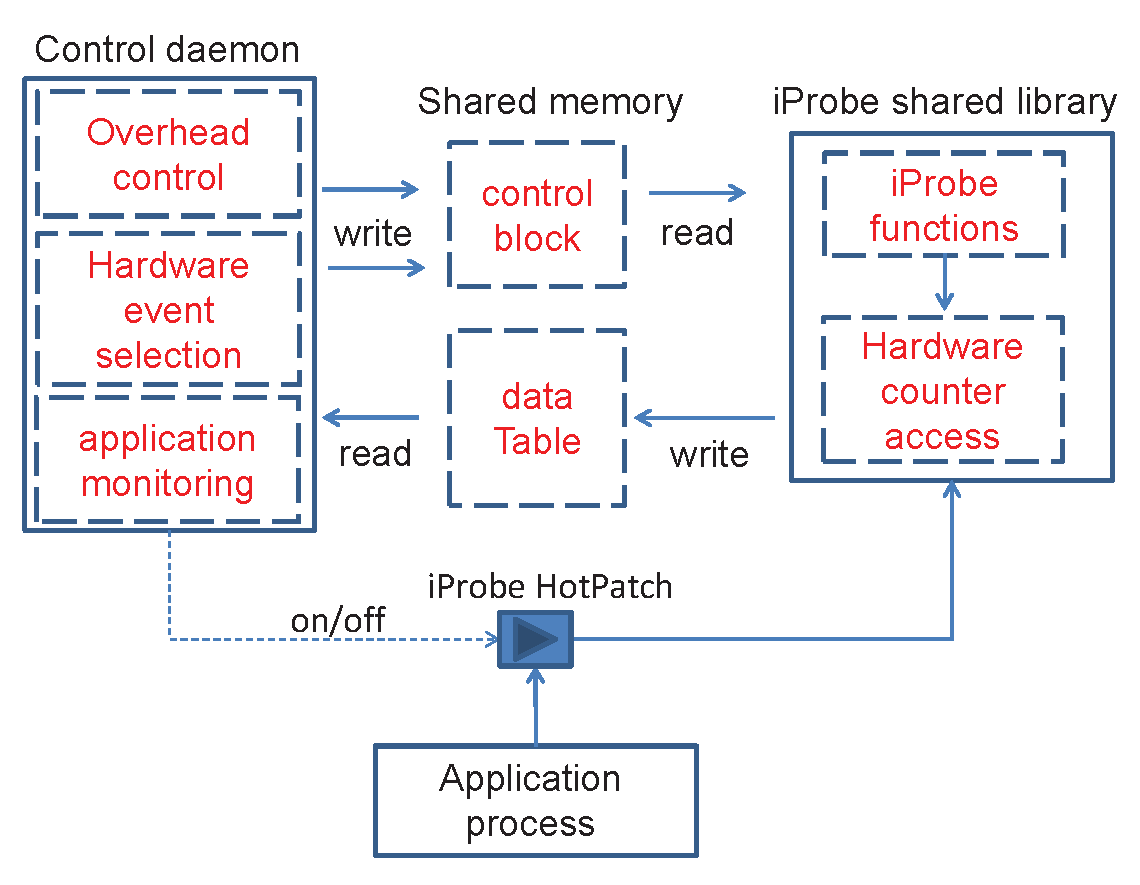
\includegraphics[width=0.8\textwidth]{iprobe/Images/sysdesign2.eps}
      \caption{Overview of \textit{FPerf}: Hardware Event Profiler based on iProbe.}
      \label{fig:implement}
    \end{center}
\end{figure}

%In this section we showcase iProbe's strength as a tool building infrastructure.  
We used iProbe to build \emph{FPerf}, an automatic function level hardware event profiler.  
FPerf uses iProbe to provide an automated way to gather hardware performance information at 
application function granularity.
%We used iProbe to build a hardware counter profiling tool called {\em FPerf}.

Hardware counters provide low-overhead access to a wealth of detailed performance information related to CPU's functional units, caches and main memory etc.
Using iProbe's all function profiling, we capture the hardware performance counters at the entry and exit of each function.
%\textit{FPerf} offers fine-grained hardware counter monitor profiling at application function level.
To control the perturbation on applications and the run-time system, \textit{FPerf} also implements a control mechanism to constraint the function profiling overhead within a budget configured by users.

Figure \ref{fig:implement} summarizes \textit{FPerf} implementation. 
It includes a control daemon and an iProbe shared library with customized instrumentation functions. 
The iProbe instrumentation functions access hardware performance counters (using PAPI\cite{papi} in the implementation) at the entry and exit of a selected target function to get the number of hardware events occurring during the function call. 
We define this process as taking one sample. 
Each selected function has a budget quota.
After taking one sample, the instrumentation functions decrease the quota for that application function by one. 
When its quota reaches zero, iProbe does not take sample anymore for that function.


The daemon process controls run-time iProbe profiling through shared memory communication.  
There are two shared data structures for this purpose: a shared control block where the daemon process passes to the iProbe instrumentation functions the profiling quota information, and a shared data table where the iProbe instrumentation functions record the hardware event information for individual function calls. 
When iProbe is enabled, i.e., the binary is HotPatched, daemon periodically collects execution data. 
We limit the total number of samples we want to collect in each time interval to restrict the overhead.  
This limitation is important because in software execution, the function call happens very frequently. 
For example, even with test data size input, the SPEC benchmarks generate 50MB-2GB trace files if we log the records for each function call. 
%Therefore, we initially assign a limitation for the total number of samples to limit the trace log size. 
%In the first 1s, when one function is called; we assign a minimum 1 sample quota for this function. 
%After that, we do not sample other calls to the function. But we keep counting the call number of the function. 
%After the initial 1s, the daemon process assigns the rest total sample quota for each selected application functions proportionally according to the previous call frequency of the functions. 
Functions that are frequently called will get more samples. 
Each selected function cannot take more samples than its assigned quota. 
The only exception happens when one function has never been called before; we assign a minimum one sample quota for each selection function. 
And we pick a function with quota that has not been used up, and decrease the quota of it by one. 
The above overhead control algorithm is a simplified Leaky Bucket algorithm~\cite{lba} originally for traffic shaping in networks. Other overhead control algorithms are also under consideration.

The control daemon also enables/disables the iProbe HotPatching based on user-defined application monitoring rules.
Essentially, this is an external control role on when and what to trace a target application with iProbe.
A full discussion of the hardware event selection scheme and monitoring rule design is beyond the scope of this paper. 

